\chapter{Estudo de Caso} \label{estudodecaso}

Como foi dito na seção \ref{cap:introducao}, o problema de como realizar o
acompanhamento de métricas de vulnerabilidade de código fonte ainda não foi bem
atacado dentro do contexto da Engenharia de Software, tendo isso em vista,
foi trabalhado um estudo de caso a fim de tentar identificar qual a melhor forma
de se acompanhar e analisar métricas de código fonte dessa natureza. O estudo
de caso realizado neste trabalho visa testar algumas hipóteses iniciais que serão apresentadas
neste mesmo capítulo, além de identificar possíveis melhorias para a continuação
do mesmo.

\section{Metodologia}

A metodologia utilizada neste estudo de caso foi feita baseada no trabalho
realizado por \emph{Meirelles} (\citeyear{meirelles2013}), onde foi levantada
uma hipótese inicial e cujo objetivo é testar tal hipótese. A definição da
hipótese inicial levantada será apresentada na subseção \ref{subsec:hipotese}.
Para o teste dessa hipótese foi selecionado um projeto de software considerado
representativo no contexto de vulnerabilidades de código fonte, que é o projeto
\emph{Linux}. Ele é a base para a grande maioria dos sistemas operacionais
disponíveis, esses sistemas são bastante utilizados por Engenheiros de Software para
o próprio desenvolvimento de software, além de ser o sistema operacional em
execução na grande maioria dos servidores de aplicações, onde geralmente
atacantes exploram vulnerabilidades ao utilizarem se de \textit{exploits}, como
foi apresentado na seção \ref{cap:metricas_vuln}.

A fim de facilitar o entendimento das atividades realizadas neste estudo de
caso, será apresentado a seguir o processo que foi seguido. Através do
fluxograma \ref{fig:processo_estudo_de_caso} pode-se ver o sequenciamento das
atividades realizadas e logo a seguir, na lista \ref{desc_processo}, o
detalhamento de cada uma delas.

\begin{figure}[h]
  \centering
  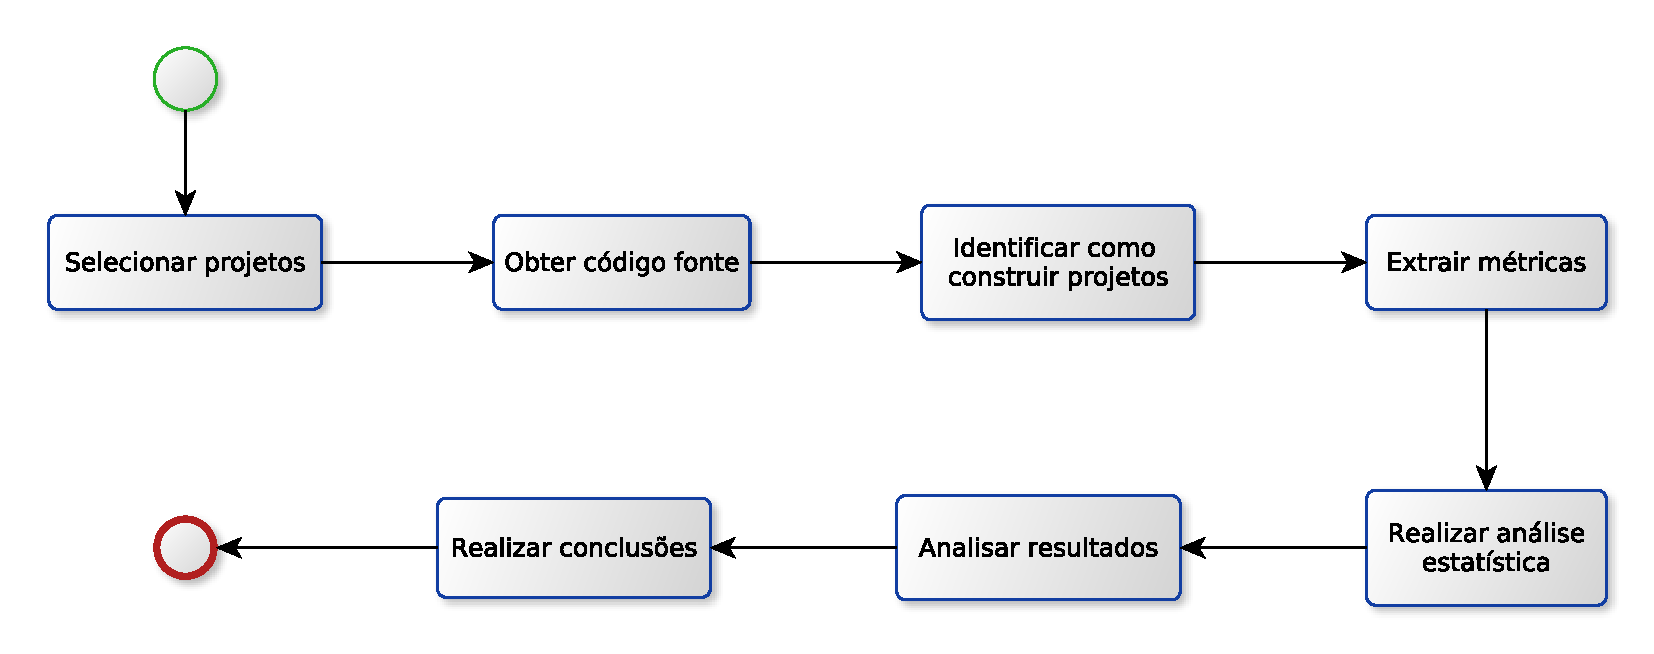
\includegraphics[width=0.9\textwidth]
      {figuras/estudo_de_caso_processo.eps}
  \caption{Processo para execução do estudo de caso}
  \label{fig:processo_estudo_de_caso}
\end{figure}

Detalhamento das atividades apresentadas no fluxograma
\ref{fig:processo_estudo_de_caso}:

\begin{enumerate}\label{desc_processo}
  \item \textbf{Selecionar projetos}: Selecionar projeto de software representativo no contexto de
    vulnerabilidades de código fonte.
  \item \textbf{Obter código fonte}: Obter código fonte do projeto selecionados. Foi utilizado o código fonte
  da última versão estável do projeto.
  \item \textbf{Identificar como construir projetos}: Identificar como construir projeto selecionado. O projeto foi contruído
    segundo as orientações da própria comunidade referente ao mesmo.
  \item \textbf{Extrair métricas}: Executar ferramenta de extração de métricas de vulnerabilidade de código
    fonte. Também foram utilizadas instruções presentes na documentação da
    ferramenta em questão.
  \item \textbf{Realizar análise estatística}: Realizar análise estatísticas sobre as métricas extraídas. Foram feitos
    tratamentos necessários das informações obtidas através da análise estática
    de código fonte, já que da maneira que foi disponibilizado pela ferramenta
    não atendia os requisitos do processo de análise estatística realizado.
  \item \textbf{Analisar resultados}: Analisar resultados gerados pela análise estatística. Essa análise foi uma atividade
    manual, analisando os gráficos e tabelas geradas pela atividade anterior um
    a um.
  \item \textbf{Realizar conclusões}: Realizar conclusões. Onde foi definido se a hipótese testada estava
    correta ou não.
\end{enumerate}

Para a realização de algumas das atividades apresentadas foram utilizadas
ferramentas para a automação das mesmas, sendo elas:

\begin{itemize}
  \item \textit{Clang Static Analyzer}, para a extração das métricas de
    vulnerabilidade de código fonte.
  \item \textit{Scripts} para adequação do formato das métricas, servindo de
    apoio a atividade de Realizar análise estatística.
  \item \textit{Scripts} para análise estatísticas, que foram elaborados no
    trabalho de \emph{Meirelles} (\citeyear{meirelles2013})
\end{itemize}

Inicialmente o intuito era utilizar a ferramenta \emph{Analizo} para a extração
das métricas de vulnerabilidade, entretanto, foram encontradas limitações na
implementação dessa \textit{feature} e por isso foi utilizada a ferramenta
\emph{Clang Static Analyzer}. A evolução dessa funcionalidade da ferramenta
\emph{Analizo} é um dos objetivos deste trabalho, como foi apresentado na seção
\ref{sec:objetivos}.

Para o entendimento completo do estudo de caso, serão apresentadas as
ferramentas utilizadas na subseção \ref{subsec:ferramentas}, iniciando pela ferramenta \emph{Analizo}, que
não foi utilizado no estudo, mas que será alvo de uma das contribuições deste
trabalho. Em seguida, serão apresentadas a ferramenta \emph{Clang Static
Analyzer}, e os \textit{Scripts} utilizados.

O teste da hipótese, desde a coleta dos dados até a análise dos resultados, serão
apresentados na subseção \ref{subsec:teste_hipotese}. Nessa subseção será
apresentado a corretude da hipótese.

\subsection{Hipótese} \label{subsec:hipotese}

%Ao iniciar este trabalho havia uma hipótese sobre como deveria se comportar as métricas de vulnerabilidades em projetos de
%software livre, baseado no trabalho de \cite{meirelles2013}. A hipótese seria que esse novo tipo de métrica se comportaria
%semelhantemente às métricas de design, onde em geral se comportariam como distribuições estatísticas de cauda longa, ou seja, 
%a média dos valores não seria representativa, e com isso, seria possível analisar os dados e fazer uma avaliação de forma 
%quantitativa. Entretanto, durante o processo empírico de desenvolvimento deste estudo de caso viu-se que a natureza das 
%métricas são diferentes. As métricas de design em sua grande maioria possuem valores significativos em todas as suas análises, 
%tendo elas valoração zero ou não, já as métricas de vulnerabilidades em grande parte das vezes, possuem valoração zero, pois 
%não possuem significado, levando em conta que as mesmas representam a quantidade de cenários de vulnerabilidades presentes no 
%código fonte em questão. Logo, nas métricas de vulnerabilidades existirão vários zeros não significativos, atrapalhando uma 
%análise similar a feita em \cite{meirelles2013}. Tendo isso em vista, decidiu-se então realizar uma análise qualitativa ao 
%invés de quantitativa.

\subsection{Ferramentas} \label{subsec:ferramentas}

\subsection{Teste da Hipótese} \label{subsec:teste_hipotese}
\subsubsection{Coleta de Dados}
\subsubsection{Análise dos Resultados}

\section{Análise Qualitativa}

%\section{Definição} \label{definicao_estudo}
%
%O objetivo dessa sessão é definir o processo inicial de execução do estudo de caso que será realizado neste trabalho, com o intuito 
%de melhor entender como deve-se dar o acompanhamento de métricas de vulnerabilidade de código fonte em projetos de software
%livre. 
%
%O processo para execução desse estudo de caso segue o fluxograma \ref{processo_estudo_de_caso}.
%
%\begin{figure}[h]
%  \centering
%  \includegraphics[width=0.8\textwidth]
%      {figuras/estudo_de_caso_processo.eps}
%  \caption{Processo para execução do estudo de caso}
%  \label{processo_estudo_de_caso}
%\end{figure}
%
%A seguir a descrição das atividades do processo apresentado no fluxograma \ref{processo_estudo_de_caso}.
%
%\begin{enumerate}\label{desc_processo}
%  \item Selecionar projetos de software que atendam os requisitos desse estudo de caso
%  \item Obter código fonte dos projetos selecionados
%  \item Identificar como construir projetos selecionados 
%  \item Executar ferramenta de extração de métricas de vulnerabilidade de código fonte
%  \item Realizar análise estatísticas sobre as métricas extraídas, incluindo tratamento dos dados se necessário
%  \item Analisar resultados gerados pela análise
%  \item Realizar conclusões
%\end{enumerate}
%
%Espera-se que esse seja um ciclo completo para execução do estudo de caso proposto, entretanto, é importante salientar que esse
%ciclo será executado uma vez, podendo ser adaptado em ciclos seguintes.
%
%\section{Ferramentas} \label{tools}
%
%A seguir serão apresentadas as ferramentas que serão utilizadas para a realização do estudo de caso definido na seção 
%\ref{definicao_estudo} e seguindo a metodologia descrita na seção \ref{metod_estudo}. As ferramentas apresentadas serão:
%
%\begin{itemize}
%  \item Analizo (\ref{analizo})
%  \item Clang (\ref{clang})
%  \item Scripts para análise estatística (\ref{scripts})
%\end{itemize}
%
%\subsection{Analizo} \label{analizo}
%
%Analizo é um conjunto de ferramentas livre, multi-linguagem (C, C++, Java), realiza análise de código fonte, é facilmente 
%extensível e disponibiliza diferentes tipos de visualização. Ele suporta a extração e cálculo de um bom número de métricas de 
%código fonte, geração de gráficos de dependência e análise de evolução do software \cite{analizo}.
%
%A seguir as funcionalidades da ferramenta Analizo \footnote{Disponível em
%\url{http://www.analizo.org/features.html}}:
%
%\begin{itemize}
%  \item Analisar código-fonte escritos em C, C ++ e Java.
%  \item Extrair métricas de código-fonte.
%  \item Extrair métricas de uma grande quantidade de projetos em lote (\textit{batch mode}).
%  \item Extrair métricas de um repositório.
%  \item Desenhar gráfico de dependências.
%  \item Analisar evolução do software (analisa-se várias versões do software e uma matriz de evolução é produzida).
%\end{itemize}
%
%Será iniciado o processo de manutenção corretiva da funcionalidade de extração de métricas de vulnerabilidade de código fonte 
%para as linguagens C e C++, para que melhor atenda as necessidades deste trabalho. Outra funcionalidade que ainda está em 
%processo de desenvolvimento é a adição do suporte da linguagem \textit{Perl}.
%
%A ferramenta Analizo é facilmente extensível, desde extratores até formas de visualização. A figura \ref{archanalizo} mostra
%como está implementada a arquitetura em camadas da ferramenta \cite{analizoartigo}. Existem basicamente cinco módulos, o 
%\textit{Core} é o modulo responsável por atividades centrais como processamento, filtros e modelos por exemplo; 
%\textit{Extractor} é o módulo que contém os extratores utilizados, atualmente existem três: \textit{Clang}, \textit{Doxyparse}
%e \textit{Sloccount}; \textit{Metrics} é o módulo que contém a lógica para cálculo de todas as métricas, hoje em dia possuindo
%37 (trinta e sete) métricas de módulo e 4 (quatro) métricas globais; \textit{Output} é o módulo que será dada a saída da 
%ferramenta, atualmente existem opções de banco de dados e arquivo CSV; \textit{Tools} é o módulo que representa várias outras
%ferramentas que podem trabalhar tanto acima do \textit{Core} quanto acima dos outros módulos.
%
%\begin{figure}[h]
%  \centering
%  \includegraphics[width=0.5\textwidth]
%      {figuras/analizo.eps}
%  \caption{Arquitetura da ferramenta Analizo}
%  \label{archanalizo}
%\end{figure}
%
%\subsection{Clang} \label{clang}
%
%Clang é um compilador \textit{front end} para as linguagens de programação C, C++ e \textit{Objective-C}. O Clang faz parte
%do projeto LLVM \textit{Open Source} e utiliza o mesmo como seu \textit{backend}. 
%
%O Clang possui algumas funcionalidades e metas disponíveis no seu respectivo
%\textit{site}\footnote{Disponível em: \url{http://clang.llvm.org}}, e
%algumas das principais metas são:
%
%\begin{itemize}
%  \item Rápida compilação e baixo uso de memória
%  \item Diagnóstico expressivos (exemplo, apresentar erros de uma maneira fácil para o usuário)
%  \item Compatibilidade com o GCC (\textit{GNU Compiler Collection})
%  \item Suportar diversos clientes (exemplo, análise estática e refatoração)
%  \item Código fonte base simples e de fácil entendimento ("\textit{hackable}")
%\end{itemize}
%
%Algumas dessas metas estão sendo atingidas, por exemplo, um experimento realizado por \cite{naroff2009} evidenciou o rápido
%tempo de compilação do Clang em comparação com o GCC. Foi feita a compilação do \textit{PostgreSQL} em computadores com as
%mesmas configuraçãoes de \textit{hardware} e o resultado obtido é expresso pela figura \ref{clang_gcc}.
%
%\begin{figure}[h]
%  \centering
%  \includegraphics[width=0.4\textwidth]
%      {figuras/clang_gcc.eps}
%  \caption{Análise de performance do Clang em comparação com o GCC}
%  \label{clang_gcc}
%\end{figure}
%
%O Clang vem sendo desenvolvido baseado na arquitetura do projeto LLVM, ele possui bibliotecas centrais e bibliotecas de 
%aplicativos, conforme é apresentado na figura \ref{clang_arch}. No contexto desse trabalho, o foco é a biblioteca de aplicativo
%\textit{Analysis}. A ideia dessa biblioteca é trazer alguns benefícios para os desenvolvedores, como o descobrimento de 
%\textit{bugs} o mais cedo possível; checar sistematicamente o código fonte; achar alguns \textit{bugs} mesmo na falta de caso
%de testes, no caso de trechos de código difíceis de serem testados \cite{kremenek2009}. 
%
%A análise estática realizada pelo Clang é inter-procedural, podendo achar inconsistências entre funções/métodos, para isso,
%é necessária a compilação do código fonte, onde nessa fase será construída a AST (\textit{Abstract Syntaxe Tree})
%\cite{kremenek2009}. Essa característica pode não ser muito atraente a primeira vista, pois para realizar a análise do código 
%fonte é necessário compila-lo, entretanto, pode ser um ponto positivo tendo em vista que a todo momento que for feita 
%construção do software a análise será feita, mesmo que essa questão tenha sido esquecida.
%
%\begin{figure}[h]
%  \centering
%  \includegraphics[width=0.4\textwidth]
%      {figuras/clang_arch.eps}
%  \caption{Arquitetura da ferramenta Clang}
%  \label{clang_arch}
%\end{figure}
%
%\subsection{\textit{Scripts} para análise estatística} \label{scripts}
%
%Poderão ser utilizados \textit{scripts}\footnote{Disponível em:
%\url{https://gitlab.com/paulormm/tese}} escritos utilizando linguagem R
%\footnote{Informações em: \url{http://www.r-project.org/}} que foram inicialmente desenvolvidos em \cite{meirelles2013}. Foi escolhida a linguagem R
%devido o seu foco e poder para a realiazação de análises estatísticas. O processo de análise estatística que será realizado
%por esses \textit{scripts} tentará identificar qual distribuição estatística melhor se encaixa nos dados referentes a 
%determinada métrica, são utilizadas as seguintes distribuições estatísticas:
%
%\begin{itemize}
%  \item Pareto
%  \item Pareto tipo 2
%  \item Exponencial
%  \item Gama
%  \item Weibull
%  \item Poison
%\end{itemize}
%
%Caso nenhuma das distribuições apresentadas consigam refletir os valores de uma determinada métrica de vulnerabilidade, os
%\textit{scripts} tentarão encontrar uma distribuição estatística que melhor se adeque. Gráficos de cada distribuição serão
%gerados como saída desse processo de análise estatística para melhor visualização dos dados. Como entrada teremos arquivos
%CSV (\textit{Comma Separeted Values}) com os valores das métricas a serem analisadas.
%
%Outro tipo de análise que poderá ser feita com essa suíte de \textit{scripts} será relacionada aos percentis das métricas.
%Dada uma amostra (ou coleção de dados), os percentis são medidas que dividem a amostra ordenada (por ordem crescente dos dados) 
%em cem (100) partes, cada uma com uma percentagem de dados aproximadamente igual. Define-se percentil k, ${Q_k}$, 
%k recebendo valores de um (1) a noventa e nove (99), como sendo o valor tal que k\% dos elementos da amostra são menores ou 
%iguais a ${Q_k}$ e os restantes (100-k)\% elementos da amostra são maiores ou iguais a ${Q_k}$ \cite{martins2013}. Os valores
%de percentis utilizados são: 
%
%\begin{multicols}{3}
%  \begin{itemize}
%    \item 1\%
%    \item 5\%
%    \item 10\%
%    \item 25\%
%    \item 50\%
%    \item 75\%
%    \item 90\%
%    \item 95\%
%    \item 99\%
%  \end{itemize}
%\end{multicols}
%
%A saída desse processo de análise estatística serão gráficos dos percentis e um arquivo texto com a quantidade de valores 
%dentro de cada intervalo de percentil.
%
%Tendo os percentis das métricas será possível fazer uma análise qualitativa, sabendo em quais faixas geralmente ocorre 
%determinados tipos de vulnerabilidades e tentar definir em qual faixa é aceitável ou não os valores das métricas de 
%vulnerabilidade de código fonte.
%
%\section{Metodologia} \label{metod_estudo}
%
%Ao iniciar este trabalho havia uma hipótese sobre como deveria se comportar as métricas de vulnerabilidades em projetos de
%software livre, baseado no trabalho de \cite{meirelles2013}. A hipótese seria que esse novo tipo de métrica se comportaria
%semelhantemente às métricas de design, onde em geral se comportariam como distribuições estatísticas de cauda longa, ou seja, 
%a média dos valores não seria representativa, e com isso, seria possível analisar os dados e fazer uma avaliação de forma 
%quantitativa. Entretanto, durante o processo empírico de desenvolvimento deste estudo de caso viu-se que a natureza das 
%métricas são diferentes. As métricas de design em sua grande maioria possuem valores significativos em todas as suas análises, 
%tendo elas valoração zero ou não, já as métricas de vulnerabilidades em grande parte das vezes, possuem valoração zero, pois 
%não possuem significado, levando em conta que as mesmas representam a quantidade de cenários de vulnerabilidades presentes no 
%código fonte em questão. Logo, nas métricas de vulnerabilidades existirão vários zeros não significativos, atrapalhando uma 
%análise similar a feita em \cite{meirelles2013}. Tendo isso em vista, decidiu-se então realizar uma análise qualitativa ao 
%invés de quantitativa.
%
%O estudo de caso inicial realizado está seguindo as atividades definidas na seção \ref{definicao_estudo}.
%
%Os requisitos para a seleção dos projetos de software que serão utilizados nesse estudo de caso são:
%
%\begin{itemize}
%  \item Possuir uma licensa de software livre (código fonte disponível)
%  \item Ser implementado utilizando a(s) linguagem(ns) C e/ou C++
%\end{itemize}
%
%Buscou-se selecionar softwares de várias naturezas a fim de entender melhor a existência ou não de variância das métricas entre 
%eles. O código fonte de cada projeto foi obtido diretamente no site oficial de cada um dos projetos selecionados.
%
%A ferramenta utilizada para extração de métricas de vulnerabilidades foi a Clang (\ref{clang}), entretanto espera-se que seja 
%utilizada a ferramenta Analizo (\ref{analizo}), sendo essa uma contribuição deste trabalho. E os \textit{scripts} apresentados 
%na seção \ref{scripts} foram utilizados para a realização da análise estatística, tendo os dados passados por um processo de 
%adequação do formato esperado pelos mesmos, já que o \textit{report} padrão do Clang é um arquivo HTML (\textit{HyperText MarkUp
%Language}) e os \textit{scripts} utilizados esperam como entrada arquivos CSV. Para essa adequação dos dados coletados foram
%utilizados \textit{scripts Perl} \footnote{Disponível em
%\url{https://github.com/lucaskanashiro/clang\_parser\_html\_to\_csv}}.
%
%A análise estatística realizada foi apenas relacionada aos percentis, não tentando determinar distribuições estatísticas para
%o acompanhamento de cada uma das métricas, vide a falta de domínio da natureza das métricas de vulnerabilidade.
%
%Ao final, como foi dito anteriormente, foi feita uma análise qualitativa dos resultados obtidos, que está apresentado na seção
%\ref{analise_estudo}
%
%\section{Análise qualitativa dos resultados obtidos} \label{analise_estudo}
%
%Os projetos selecionados inicialmente para realizar este estudo de caso foram os seguintes, levando em consideração os 
%requisitos apresentados na seção \ref{metod_estudo}:
%
%\begin{multicols}{2}
%  \begin{itemize}
%    \item Bash
%    \item Blender
%    \item FFmpeg
%    \item Firefox
%    \item Gstreamer
%    \item Inetutils
%    \item Openssh
%    \item Openssl
%    \item Python2.7
%    \item Ruby-2.1
%  \end{itemize}
%\end{multicols}
%
%Os gráficos gerados a partir da análise de percentis podem ser visualizados
%no anexo\ref{anex:percentis}.
%
%Devido a diferente natureza das métricas de vulnerabilidade, existem alguns pontos importantes que devem ser apresentados com
%relação aos resultados obtidos na extração das métricas de vulnerabilidade:
%
%\begin{itemize}
%  \item São apresentados apenas arquivos que apresentaram algum cenário de vulnerabilidade em seu conteúdo, os demais são
%    omitidos.
%  \item Mesmo um arquivo tendo apresentado algum cenário de vulnerabilidade, geralmente, a grande maioria das métricas 
%    relacionadas possuem valoração igual a zero;
%\end{itemize}
%
%Devido ao fato apresentado anteriormente, a análise dos percentis de algumas métricas em determinados projetos não será 
%representativa, pois possuem valoração zero em todos os casos, apresentando gráficos de percentis com retas sobre o valor 
%zero. Isso pode ser visto em alguns dos gráficos no anexo
%\ref{anex:percentis}, como o gráfico \ref{graphic:asom}.
%
%Entretanto, ao descartar as métricas de vulnerabilidades de código fonte com
%valor não significativo (iguais a zero), pode-se perceber que praticamente
%todas possuem uma tendência a se concentrarem entre percentis de 80\% e 99\%, mostrando que se
%comportam de maneira similar.
%
%Contudo, percebeu-se que analisar métricas de vulnerabilidade de código fonte
%seguindo esse viés também não resultaria em algo satisfatório, devido a grande
%maioria das métricas não possuírem valor representativo, atrapalhando assim
%a análise. Havia maior existência de métricas com valores não
%significativos do que propriamente significativos, não dando o valor e
%confiança esperada ao resultado obtido.
%
%\section{Conclusão}
